% --------------------------------------------------------------------------
% A LaTeX / Beamer example template that I put together  
% for my PLSC 502 students in 2024.
%
% Christopher Zorn
% August 25, 2024
%
% The actual content of the slides starts somewhere
% around line 250; everything before that is preamble.
%
% This entire thing is a peek inside my warped mind, so 
% tread with caution.
% --------------------------------------------------------------------------
\documentclass[10pt]{beamer}
%----- Beamer Options --------------------
%
% Theme examples are HERE:   http://www.hartwork.org/beamer-theme-matrix/
%
\setbeamercolor{title}{fg=black}
\setbeamercolor{title}{bg=white}
\setbeamercolor{frametitle}{fg=black}
\setbeamercolor{frametitle}{bg=white}
\setbeamercolor{enumerate items}{fg=black}
\setbeamertemplate{enumerate item}{\insertenumlabel.}
\setbeamertemplate{enumerate subitem}{\insertenumlabel.\insertsubenumlabel}
\setbeamercolor{itemize item}{fg=black} 
\setbeamercolor{itemize item}{fg=black} % all frames will have red bullets
\setbeamercolor{itemize subitem}{fg=black} % all frames will have red bullets
\setbeamercolor{itemize subsubitem}{fg=black} % all frames will have red bullets
\setbeamercolor{enumerate item}{fg=black} 
\setbeamercolor{enumerate subitem}{fg=black} % all frames will have red bullets
\setbeamercolor{enumerate subsubitem}{fg=black} % all frames will have red bullets
\setbeamertemplate{navigation symbols}{}
\setbeamertemplate{footline}[frame number]
\setbeamertemplate{itemize items}[default]
\setbeamertemplate{enumerate items}[default]
% Theme & Colors:
\usetheme{Pittsburgh}
\usecolortheme{dove}
%\usepackage{beamerthemesplit} % new
%-----------------------------------------------------------------------
%  Packages   ------------------------------------------------------
%-----------------------------------------------------------------------
\usepackage{amsmath}
\usepackage{amssymb}
\usepackage{amsfonts}
\usepackage{pifont}
\usepackage{bm}
\usepackage{ifsym}
%\usepackage[all]{xy}
\usepackage{color}
\usepackage{multicol}
\usepackage{tabularx}
%\usepackage[abbr]{harvard}
%\usepackage{lscape}
%\usepackage[pdftex]{graphicx}
%\usepackage{fullpage}
%\usepackage{longtable}
%\usepackage[pdftex,bookmarks,colorlinks,breaklinks]{hyperref}  % PDF hyperlinks, with coloured links
%\usepackage{cite}
\usepackage{natbib}
%\usepackage{portland}
\usepackage{multirow}
\usepackage{subeqnarray,amsmath}
%\usepackage[top=1in,bottom=1in,left=1in,right=1in]{geometry}
%----------------------------------------------------------------------
%  Fonts  -----------------------------------------------------------
%----------------------------------------------------------------------
%\usepackage{cmbright} % [sans-serif for both math and text!]
%\usepackage{bookman}
%\usepackage{times}
%\usepackage{newcent}
%\usepackage{palatino}
%\usepackage{palatcm}
%\usepackage{lmodern} % math, rm, ss, tt
%\usepackage[T1]{fontenc}
%\renewcommand{\familydefault}{pag}  % Adobe AvantGarde
%\renewcommand{\familydefault}{pnc}  % Adobe New Century Schoolbook
%\renewcommand{\familydefault}{pbk}   % Bookman
%\renewcommand{\familydefault}{bch}  % Charter
%\renewcommand{\familydefault}{comic}   % Comic
%\renewcommand{\familydefault}{cmdh}   % CM Dunhill
%\renewcommand{\familydefault}{cmfib}   % CM Fibonacci
%\renewcommand{\familydefault}{cmfr}   % CM Funny Roman
%\renewcommand{\familydefault}{cmss} % CM Sans Serif
%\renewcommand{\familydefault}{cmtt}   % CM Typewriter
%\renewcommand{\familydefault}{ccr}   % Concrete Roman -- ugly...
%\renewcommand{\familydefault}{pcr}  % Courier
%\renewcommand{\familydefault}{phv}  % Helvetica
%\renewcommand{\familydefault}{ppl}   % Palatino
%\renewcommand{\familydefault}{ptm}   % Times
%\renewcommand{\familydefault}{put}  % Utopia
%\renewcommand{\familydefault}{pzc}  % Zapf Chancery
%--------------------------------------------------------------------------
% Other preferences ------------------------------------------------
%--------------------------------------------------------------------------
%\pagestyle{plain}
%\clubpenalty=9999
%\widowpenalty=9999
%\displaywidowpenalty=9999
%--------------------------------------------------------------------------
% Fuzzy stuff ----------------------------------------------------------
%--------------------------------------------------------------------------
%\hfuzz6pt % Don't bother to report over-full boxes < 6pt
%\vfuzz6pt % Don't bother to report over-full boxes < 6pt
%--------------------------------------------------------------------------
% Bibliography thing ------------------------------------------------
%--------------------------------------------------------------------------
\renewcommand{\bibitem}{\vskip 10pt\par\hangindent\parindent\hskip-\parindent}
%--------------------------------------------------------------------------
% HTML Things... ----------------------------------------------------
%--------------------------------------------------------------------------
\definecolor{dullmagenta}{rgb}{0.4,0,0.4}   % #660066
\definecolor{darkblue}{rgb}{0,0,0.4}
\definecolor{darkgreen}{rgb}{0,0.4,0}
\definecolor{PSU}{rgb}{0,0.16,0.47}
\definecolor{GSERM}{rgb}{0,0.477,0.246}
\hypersetup{colorlinks=TRUE,linkcolor=,citecolor=GSERM,filecolor=GSERM,urlcolor=GSERM} % coloured links
%--------------------------------------------------------------------------
% Full-Sized Footnotes ---------------------------------------------
%--------------------------------------------------------------------------
%\let\footnotesize\normalsize
%--------------------------------------------------------------------------
%-=-=-=-=-=-=-=-=-=-=- TIKZ Stuff...=-=-=-=-=-=-=-=-=-=-=-=-=-=-=-=-=
\usepackage{tikz}
\usetikzlibrary{shapes.geometric, arrows}
\tikzstyle{startstop} = [rectangle, rounded corners, minimum width=3cm, minimum height=1cm,text centered, draw=black, fill=white!30]
\tikzstyle{io} = [trapezium, trapezium left angle=70, trapezium right angle=110, minimum width=3cm, minimum height=1cm, text centered, draw=black, fill=grey!30]
\tikzstyle{process} = [rectangle, minimum width=2cm, minimum height=1cm, text centered, draw=black, fill=white!30]
\tikzstyle{decision} = [diamond, minimum width=2cm, minimum height=1cm, text centered, draw=black, fill=white!30]
\tikzstyle{whitespace} = [rectangle, minimum width=2cm, minimum height=1cm, text centered, text width = 3cm, draw=white, fill=white]
\tikzstyle{arrow} = [thick,->,>=stealth]
\tikzset{>=latex}
%--------------------------------------------------------------------------
% A Little Math --------------------------------------------------------
%--------------------------------------------------------------------------
\newcommand{\norm}[1]{\left\Vert#1\right\Vert}
\newcommand{\abs}[1]{\left\vert#1\right\vert}
\newcommand{\set}[1]{\left\{#1\right\}}
\newcommand{\bhat}{\boldsymbol{\hat{\beta}}}
\newcommand{\eps}{\varepsilon}
\newcommand{\To}{\longrightarrow}
%--------------------------------------------------------------------------
%      -modelsummary- things...     -------------------------------
%--------------------------------------------------------------------------
\usepackage{booktabs}
\usepackage{caption}
\usepackage{longtable}
%\usepackage{graphicx}
\usepackage{codehigh}
\usepackage{xcolor}
\usepackage{siunitx}
\usepackage{tabularray}
\usepackage{float}
\usepackage{graphicx}
\usepackage[normalem]{ulem}
\UseTblrLibrary{booktabs}
\newcommand{\tinytableTabularrayUnderline}[1]{\underline{#1}}
\newcommand{\tinytableTabularrayStrikeout}[1]{\sout{#1}}
\NewTableCommand{\tinytableDefineColor}[3]{\definecolor{#1}{#2}{#3}}
%\newcolumntype{d}{S[
%    input-open-uncertainty=,
%    input-close-uncertainty=,
%    parse-numbers = false,
%    table-align-text-pre=false,
%    table-align-text-post=false
% ]}
%--------------------------------------------------------------------------
% Listing shortcuts & details... ------------------------------------
%--------------------------------------------------------------------------
\newcommand{\nin}{\noindent}
\newcommand{\non}{\nonumber}
\newcommand{\beq}{\begin{equation}}
\newcommand{\eeq}{\end{equation}}
\newcommand{\bea}{\begin{eqnarray}}
\newcommand{\eea}{\end{eqnarray}}
\newcommand{\be}{\begin{enumerate}}
\newcommand{\ee}{\end{enumerate}}
\newcommand{\bi}{\begin{itemize}}
\newcommand{\ei}{\end{itemize}}
\newcommand{\bverb}{\begin{verbatim}}
\newcommand{\everb}{\end{verbatim}}
\newcommand{\bv}{\begin{verbatim}}
\newcommand{\ev}{\end{verbatim}}
\newcommand{\+}{\item}
\newcommand{\?}{\item[$\cdot$]}
\newcommand{\bl}{\begin{large}}
\newcommand{\el}{\end{large}}
\newcommand{\bL}{\begin{Large}}
\newcommand{\eL}{\end{Large}}
\newcommand{\subs}{\subsection*}
\newcommand{\subss}{\subsubsection*}
\newcommand{\Prob}{\text{Pr}}
%\renewcommand{\labelitemi}{$\bullet$}
%\renewcommand{\labelitemii}{$\circ$}
%\renewcommand{\labelitemiii}{$\cdot$}
\newcommand{\upone}{\vspace*{-10pt}}
\newcommand{\uptwo}{\vspace*{-20pt}}
\newcommand{\upthree}{\vspace*{-30pt}}
%--------------------------------------------------------------------------
% Math boldface shortcuts, etc. ----------------------------------
%--------------------------------------------------------------------------
\newcommand{\X}{\mathbf{X}}
\newcommand{\Y}{\mathbf{Y}}
\newcommand{\Z}{\mathbf{Z}}
\newcommand{\N}{\mathbf{N}}
\newcommand{\I}{\mathbf{I}}
\newcommand{\V}{\mathbf{V}}
\newcommand{\W}{\mathbf{W}}
\newcommand{\U}{\mathbf{U}}
\newcommand{\R}{\mathbf{R}}
\newcommand{\A}{\mathbf{A}}
\newcommand{\B}{\mathbf{B}}
\newcommand{\C}{\mathbf{C}}
\newcommand{\T}{\mathbf{T}}
\renewcommand{\O}{\mathbf{O}}
\newcommand{\Q}{\mathbf{Q}}
\renewcommand{\P}{\mathbf{P}}
\renewcommand{\H}{\mathbf{H}}
\newcommand{\uu}{\mathbf{u}}
\newcommand{\E}{\mathbf{e}}
\newcommand{\x}{\mathbf{x}}
\newcommand{\w}{\mathbf{w}}
\newcommand{\vv}{\mathbf{v}}
\newcommand{\0}{\mathbf{0}}
\newcommand{\1}{\mathbf{1}}
\newcommand{\e}{\text{exp}}
\newcommand{\Beta}{\boldsymbol{\beta}}
\newcommand{\Mu}{\boldsymbol{\mu}}
\newcommand{\Eta}{\boldsymbol{\eta}}
\newcommand{\BTheta}{\boldsymbol{\theta}}
\newcommand{\THETA}{\boldsymbol{\Theta}}
\newcommand{\GAMMA}{\boldsymbol{\Gamma}}
\newcommand{\OMEGA}{\boldsymbol{\Omega}}
\newcommand{\red}{\textcolor{red}}
\newcommand{\green}{\textcolor{green}}
\newcommand{\yellow}{\textcolor{yellow}}
\newcommand{\blue}{\textcolor{blue}}
\newcommand{\PSU}{\textcolor{PSU}}
\newcommand{\Stata}{\textsf{Stata}~}
\newcommand{\SAS}{\textsf{SAS}~}
\newcommand{\RR}{\textsf{R}~}
% ---------------------------------------------------------------
%  Back-up slides thing...
\newcommand{\backupbegin}{
   \newcounter{framenumberappendix}
   \setcounter{framenumberappendix}{\value{framenumber}}
}
\newcommand{\backupend}{
   \addtocounter{framenumberappendix}{-\value{framenumber}}
   \addtocounter{framenumber}{\value{framenumberappendix}} 
}
% ---------------------------------------------------------------

% ---------------------------------------------------------------
\begin{document}
%\renewcommand{\inserttotalframenumber}{53} % <-- edit if you want to have slides "after" the last one... 
% ---------------------------------------------------------------

\title{\huge {\bf PLSC 502} \\ \LaTeX~Beamer Template}
%\author{Author}
\date{August 25, 2024}

\frame{\titlepage}  % <-- makes the title page, naturally

%\frame{\frametitle{Table of contents}\tableofcontents}

% ---------------------------------------------------------------% ---------------------------------------------------------------% ------------------------------------------------
\section{Introduction}
% ---------------------------------------------------------------% ---------------------------------------------------------------% ------------------------------------------------

% ---------------------------------------------------------------% ---------------------------------------------------------------% ------------------------------------------------
\begin{frame}[fragile] \frametitle{Texts and Lists}

\nin This is some basic text.

\bi

\+ These are elements...

\+ ...in an unordered list...

\+ ... including
   \bi
   \? ...an
   \? ...unordered
   \? ...sublist. 
   \ei
\ei

\be
\+ And this is a 
\+ numbered list.
\ee

\be
\+[1.] (The list looks better if 
\+[2.] if you number it this way.)
\ee


\end{frame}


% ---------------------------------------------------------------% ---------------------------------------------------------------% ------------------------------------------------
\begin{frame}[fragile] \frametitle{Math and Equations}

\nin We write math in \LaTeX~because it's easy and it looks cool. \\

\medskip

\nin This template has a lot of shortcuts for commonly-used terms:  \\

\medskip

$\Beta, \Mu. \Eta, \BTheta, \THETA, \GAMMA, \OMEGA, \X, \Y, \Z, \N, \W, \V, \U, \R, \A, \B, \C, \T, \O, \P, \H, \Q$, \\
$\uu, \E, \x, \vv, \0, \1$, etc. \\

\medskip

\nin Equations:

\beq
\non \Beta = (\X'\X)^{-1}\X'\Y
\eeq

\nin ... and arrays

\bea
\non \frac{\partial E(Y)}{\partial X}      &=&       \beta \\
\non                                           &   \approx &  0
\eea

\nin ...are also pretty easy.


\end{frame}

% ---------------------------------------------------------------% ---------------------------------------------------------------% ------------------------------------------------
\begin{frame}[fragile] \frametitle{A Figure (OK, it's a cat)}

\upone

\begin{center}
\resizebox{3in}{!}{\includegraphics{CatEmbed.pdf}}
\end{center}

\end{frame}


% ---------------------------------------------------------------% ---------------------------------------------------------------% ------------------------------------------------
\begin{frame}[fragile] \frametitle{Multiple Columns}

\upone

\begin{columns}

\begin{column}{0.4\linewidth}

\resizebox{1.5in}{!}{\includegraphics{CatEmbed.pdf}}

\end{column}

\begin{column}{0.6\linewidth}

\nin There are two columns here. The one on the left has a figure; the one on the right happens to be text.

\bigskip

\bi
\+ Columns can include a list

\+ like this
\ei

\bigskip

\nin Or an equation:

\beq
\non y=mx+b
\eeq

\end{column}

\end{columns}

%------------------------------------------------
\end{frame}




% ---------------------------------------------------------------% ---------------------------------------------------------------% ------------------------------------------------
\begin{frame}[fragile] \frametitle{Directed Graphs, etc.\ (using TIKZ)}


\begin{center}
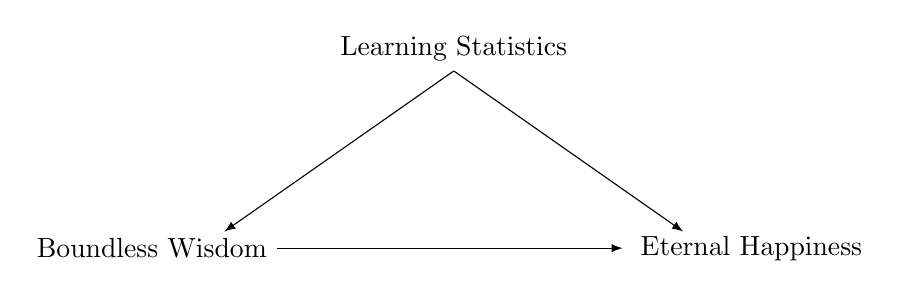
\begin{tikzpicture}[scale=1.5]
%arrows
\draw[-latex, shorten >=3pt]  (0,1) -- (3,1);
\draw[-latex, shorten >=3pt]  (1.5, 2.5) -- (-0.5,1.1);
\draw[-latex, shorten >=3pt] (1.5,2.5) -- (3.5,1.1);
\node[left] at (0,1) {Boundless Wisdom};
%\draw[fill] (3,1) circle (2pt);
\node[right] at (3,1) {Eternal Happiness};
%\draw[fill] (1.5,2.5) circle (2pt);
\node[above] at (1.5,2.5) {Learning Statistics};
\end{tikzpicture}
\end{center}

%------------------------------------------------
\end{frame}


% ---------------------------------------------------------------% ---------------------------------------------------------------% ------------------------------------------------
\begin{frame}[fragile,shrink=10] \frametitle{The Same Table, Twice}



\begin{center}
This is a table... \\
\smallskip
\begin{tabular}{lccc}
\hline \hline
Variable & Bad & Not Bad & Actually Good \\
\hline
(Intercept) &   1.23   &   0.75    &   22.31   \\
                  & (4.45)  & (1.91)    &  (0.17) \\
Main $X$   &  -0.003 &  0.46    &  5,38    \\
                  & (9.08)  & (0.23)    &  (0.04) \\
                 &            &              &                \\
$N$          & Some  &  Lots     &   $\infty$  \\
$R^{2}$    & too smol & Nice & Very nice! \\
\hline \hline
\end{tabular}
\end{center}

\bigskip

\begin{center}
This is a table... \\
\smallskip
\begin{tabular}{lccc}
\hline \hline
Variable & Bad & Not Bad & Actually Good \\
\hline
(Intercept) &   1.23   &   0.75    &   22.31   \\
                  & (4.45)  & (1.91)    &  (0.17) \\
Main $X$   &  -0.003 &  0.46    &  5,38    \\
                  & (9.08)  & (0.23)    &  (0.04) \\
                 &            &              &                \\
$N$          & Some  &  Lots     &   $\infty$  \\
$R^{2}$    & too smol & Nice & Very nice! \\
\hline \hline
\end{tabular}
\end{center}

\end{frame}

% ---------------------------------------------------------------% ---------------------------------------------------------------% ------------------------------------------------
\begin{frame}[fragile] 

\bigskip

\begin{center}
\begin{huge}
\textbf{The End}
\end{huge}
\end{center}


\appendix         % <-- Start the appendix
\backupbegin   % <-- Renumber things

\end{frame}


% ---------------------------------------------------------------% ---------------------------------------------------------------% ------------------------------------------------
\begin{frame}[fragile] \frametitle{An ``Appendix''}

\nin This is a backup / ``appendix'' slide. \\

\bigskip

\nin Note the page number.

\end{frame}


\backupend   % <-- End renumbering

% ---------------------------------------------------------------% ---------------------------------------------------------------% -------------------------------------------------
% ---------------------------------------------------------------% ---------------------------------------------------------------% -------------------------------------------------
\end{document}
% ---------------------------------------------------------------% ---------------------------------------------------------------% -------------------------------------------------
% ---------------------------------------------------------------% ---------------------------------------------------------------% -------------------------------------------------


% ---------------------------------------------------------------% ---------------------------------------------------------------% ------------------------------------------------
\begin{frame}[fragile] \frametitle{\LaTeX~Code Graveyard}

\nin This is a slide that doesn't even appear in the slides. \\

\bigskip

\nin It's here because the space after \texttt{end{document}} can be a great spot to store code + content that you may not need in the document now, but will possibly want later.

\end{frame}


